\documentclass[tikz,border=6pt]{standalone}
\usepackage[T1]{fontenc}
\usepackage[utf8]{inputenc}
\usepackage{pgfplots}
\usepgfplotslibrary{groupplots}
\usetikzlibrary{calc}
\pgfplotsset{compat=1.18}
\begin{document}
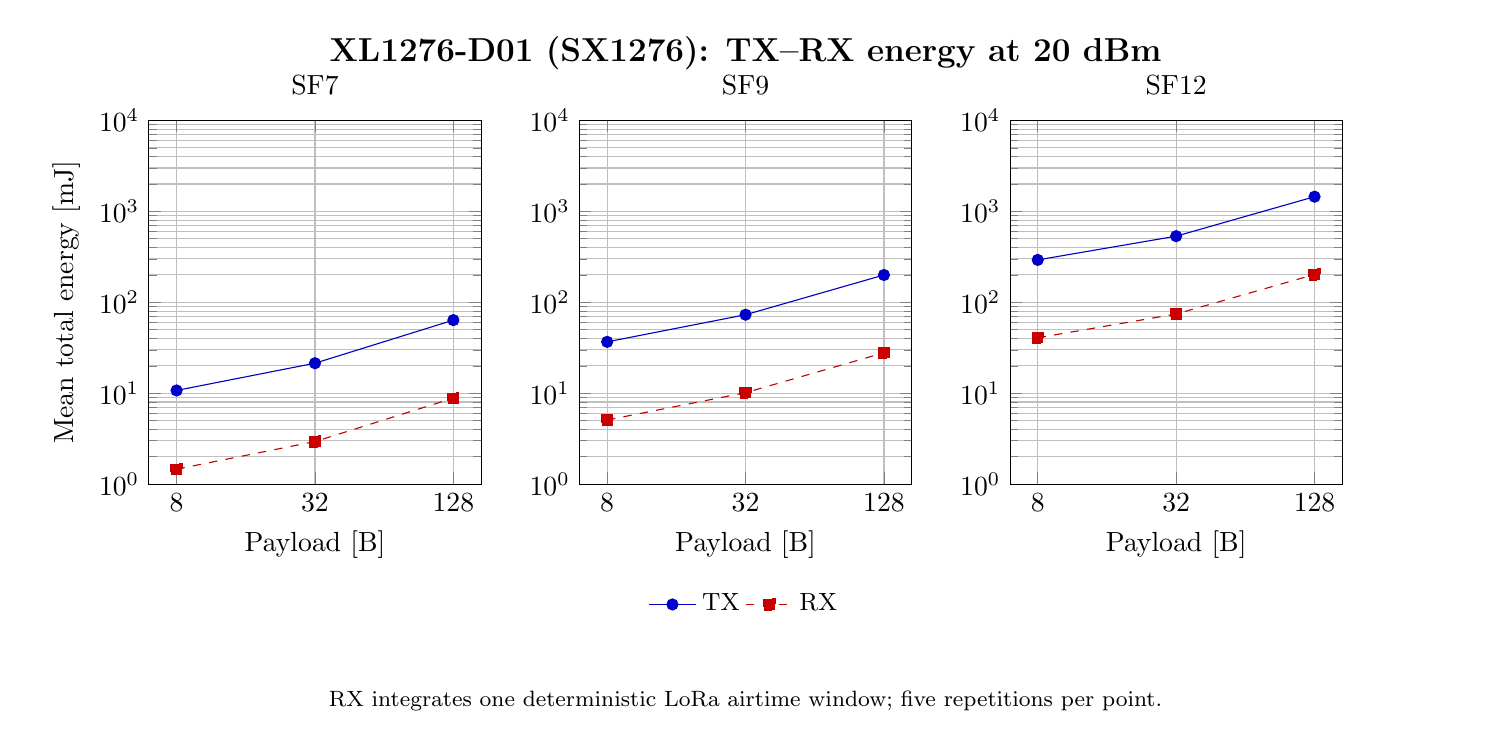
\begin{tikzpicture}
\begin{groupplot}[/pgf/number format/use comma, group style={group size=3 by 1, horizontal sep=1.25cm},
  width=5.8cm,height=6.2cm,xmode=log,log basis x=2,ymode=log,log basis y=10,ymin=1,ymax=10000,
  xtick={8,32,128},xticklabels={8,32,128},grid=both,xlabel={Payload [B]},
  legend style={draw=none,fill=none,font=\small,at={(0.5,-0.27)},anchor=north,legend columns=-1}]
% TX--RX energy
\nextgroupplot[title={SF7},ylabel={Mean total energy [mJ]}]
\addplot+[blue!75!black,solid,mark=*,error bars/.cd,y dir=both,y explicit] coordinates {(8,10.7129874) +- (0,0.0393152079) (32,21.3522876) +- (0,0.0766455207) (128,63.6052744) +- (0,0.195217459)};
\addplot+[red!75!black,dashed,mark=square*,error bars/.cd,y dir=both,y explicit] coordinates {(8,1.45866925) +- (0,0.00136651658) (32,2.93425773) +- (0,0.00097039791) (128,8.8259507) +- (0,0.0119274916)};
\nextgroupplot[title={SF9}]
\addplot+[blue!75!black,solid,mark=*,error bars/.cd,y dir=both,y explicit] coordinates {(8,36.6743408) +- (0,0.101582767) (32,72.9103052) +- (0,0.282399864) (128,199.507278) +- (0,0.520631482)};
\addlegendentry{TX}
\addplot+[red!75!black,dashed,mark=square*,error bars/.cd,y dir=both,y explicit] coordinates {(8,5.06518363) +- (0,0.00521767691) (32,10.1218945) +- (0,0.0127548942) (128,27.7961175) +- (0,0.0214273474)};
\addlegendentry{RX}
\nextgroupplot[title={SF12}]
\addplot+[blue!75!black,solid,mark=*,error bars/.cd,y dir=both,y explicit] coordinates {(8,292.279342) +- (0,0.840966523) (32,533.160977) +- (0,0.602460535) (128,1449.53109) +- (0,1.3158541)};
\addplot+[red!75!black,dashed,mark=square*,error bars/.cd,y dir=both,y explicit] coordinates {(8,40.6236395) +- (0,0.0600231456) (32,74.2181615) +- (0,0.0634351322) (128,202.173587) +- (0,0.0629388361)};
\end{groupplot}
\node[font=\bfseries\large] at ($(group c2r1.north)+(0,0.85cm)$) {XL1276-D01 (SX1276): TX--RX energy at 20 dBm};
\node[font=\footnotesize,align=center,text width=18cm] at ($(group c2r1.south)+(0,-2.75cm)$) {RX integrates one deterministic LoRa airtime window; five repetitions per point.};
\end{tikzpicture}
\end{document}
